% Provenance (never printed): see sources/outline_sources.md (Year 1: the general
% circulation of the atmosphere, Hadley, Ferrel and polar cells, the ITCZ, Walker cells,
% jet streams, the geostrophic wind, depressions and anticyclones). Exercise and problem
% values in the Book 3 scratch calculator calc/ch28.py; figures from
% figdata/bachelor-1/angular_momentum_wind.py, weather_map.py (an invented map) and
% general_circulation.py (NCEP-NCAR Reanalysis 1, long-term means 1991-2020, datasets
% bachelor-1-ncep-{uwnd-p,vwnd-p,uwnd-sfc,slp,prate-monthly}).
% Physics owns the Coriolis force and the hydrostatic relation (recalled). Book 1 (g8) gave
% the global winds, the convection cell, depressions and anticyclones, isobars and the
% rotation of the wind around them, in words: re-founded here with forces and data.
% ENSO and the monsoons are the Year 2 volume's; the thermal wind the Year 3 volume's.
\chapter{The General Circulation of the Atmosphere}\label{ch:b1:atmospheric-circulation}

The sailing ships that crossed from Europe and Africa to the Americas relied on the
\omterm{def:b1:atmospheric-circulation:winds}{trade winds}, steady easterlies of the tropics. Nearer the equator, within about five
degrees of it, the same winds died away, in the belt of calms and persistent
showers that sailors called the doldrums. Far above both, about nine kilometres
up, narrow rivers of air called \omterm{def:b1:atmospheric-circulation:jet}{jet streams} can blow at more than
\qty{440}{km/h}. This chapter explains the three: why air moving over a rotating
planet ends up blowing along the isobars rather than across them, how the
surplus of the tropics drives a great overturning cell on each side of the equator,
and why the air that leaves the equator aloft turns into a westerly jet.
% ledger: nos:trade-winds, nos:doldrums, noaajs:jet

\begin{omfigure}
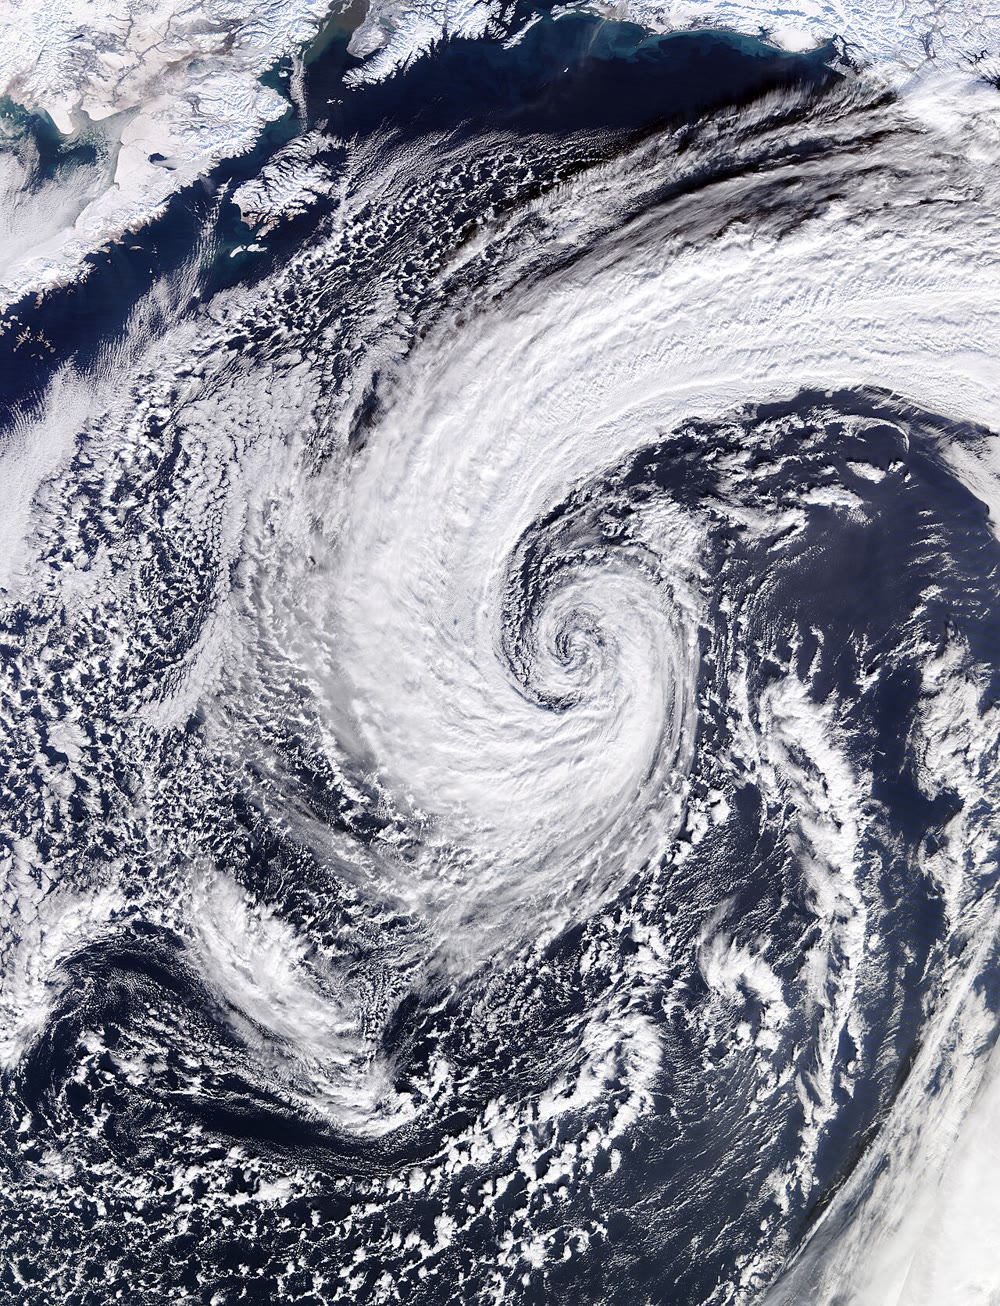
\includegraphics[width=0.5\linewidth]{images/book3/b1-alaska-low.jpg}

{\small An extratropical \omterm{def:b1:atmospheric-circulation:cyclone}{cyclone} over the Gulf of Alaska on 28 January 2018, seen
by the MODIS instrument from orbit; the snow-covered coast of Alaska is at the top
left, and north is roughly up. The bands of cloud spiral anticlockwise into the
centre, as the air of a Northern-Hemisphere depression does. (NASA, MODIS/LANCE,
public domain, via Wikimedia Commons.)}
\label{fig:b1:atmospheric-circulation:alaska}
\end{omfigure}
% ledger: commons:alaska-low, nws:cyclone

\begin{recall}
The physics volumes give the hydrostatic relation and the Coriolis force: in a
frame that rotates with angular velocity $\vec\Omega$, a body of mass $m$ moving
at velocity $\vec v$ relative to the frame feels the fictitious force
$-2m\,\vec\Omega\times\vec v$, at right angles to its motion. For the Earth,
$\Omega = 2\pi/T_\star$ with the sidereal day $T_\star = \qty{23.9345}{h}$, that is
$\Omega = \qty{7.292e-5}{rad.s^{-1}}$. Book~1 described the global winds (the \omterm{def:b1:atmospheric-circulation:winds}{trade
winds}, the \omterm{def:b1:atmospheric-circulation:winds}{westerlies}, the polar easterlies), the convection cell, depressions and
\omterm{def:b1:atmospheric-circulation:cyclone}{anticyclones}, the isobars of a weather map, and the turning of the wind around the
centres. \Cref{ch:b1:fluid-envelopes-structure} gave the \omterm{def:b1:fluid-envelopes-structure:standard-atmosphere}{standard atmosphere} and the
\omterm{def:b1:fluid-envelopes-structure:lapse-rate}{dry adiabatic lapse rate}, and \cref{ch:b1:radiation-heat-transport} the poleward
heat transport that the circulation carries.
% ledger: earth:Trot, nws:coriolis
\end{recall}

\section{Forces on moving air}\label{sec:b1:atmospheric-circulation:forces}

A parcel of air is pushed by the pressure of the air around it, pulled by gravity,
slowed by friction near the ground, and, as seen from the rotating Earth, deflected
by the Coriolis force. Gravity and the vertical pressure force balance each other
almost exactly: this is the hydrostatic relation. The weather is made by the forces
that remain in the horizontal.

\begin{definition}[Pressure-gradient force]\label{def:b1:atmospheric-circulation:pgf}
The \emph{pressure-gradient force}\index{pressure-gradient force} is the net force
exerted on a parcel of fluid by the pressure of the fluid around it. Per unit mass it
is $-(1/\rho)\nabla p$, where $\rho$ is the density and $\nabla p$ the pressure
gradient: it points from high towards low pressure, across the isobars.
\end{definition}
% ledger: nws:geostrophic

\begin{proposition}[The pressure-gradient force]\label{prop:b1:atmospheric-circulation:pgf}
On a parcel of volume $\mathrm dV$ and density $\rho$, the pressure of the
surrounding fluid exerts the force $-\nabla p\,\mathrm dV$, an acceleration
$-(1/\rho)\nabla p$.
\end{proposition}

\begin{proof}
Take a small box with edges $\mathrm dx$, $\mathrm dy$, $\mathrm dz$ along the
axes. On its face at $x$, the pressure pushes in the $+x$ direction with the force
$p(x)\,\mathrm dy\,\mathrm dz$; on its face at $x + \mathrm dx$, in the $-x$
direction with $p(x + \mathrm dx)\,\mathrm dy\,\mathrm dz$. The net force along
$x$ is $[p(x) - p(x + \mathrm dx)]\,\mathrm dy\,\mathrm dz = -(\partial p/\partial
x)\,\mathrm dV$, and likewise along $y$ and $z$. The total is $-\nabla p\,
\mathrm dV$; dividing by the mass $\rho\,\mathrm dV$ gives the acceleration.
\end{proof}

A uniform pressure exerts no net force: only its differences push. On a weather
map the horizontal gradient is read from the isobars: its size is the pressure step
between two isobars divided by their distance. For isobars \qty{4}{hPa} apart and
\qty{400}{km} apart at sea level, where $\rho \approx \qty{1.225}{kg.m^{-3}}$, the
acceleration is $400/(1.225 \times \num{4e5}) = \qty{8.2e-4}{m.s^{-2}}$, less than
a ten-thousandth of $g$, yet enough to bring air from rest to \qty{10}{m/s} in
three and a half hours.
% ledger: ussa76:sea-level

The air feels the Coriolis force because it is observed from the turning Earth. Its
horizontal part depends on the \omterm{def:b1:spherical-astronomy:geographic}{latitude} through a single number.

\begin{definition}[Coriolis parameter]\label{def:b1:atmospheric-circulation:coriolis-parameter}
The \emph{Coriolis parameter}\index{Coriolis parameter} at \omterm{def:b1:spherical-astronomy:geographic}{latitude} $\varphi$ is
$f = 2\Omega\sin\varphi$, where $\Omega$ is the angular velocity of the Earth. It is
positive in the Northern Hemisphere, negative in the Southern, zero at the equator,
and largest at the poles, $2\Omega = \qty{1.458e-4}{s^{-1}}$.
\end{definition}
% ledger: earth:Trot

\begin{proposition}[Horizontal Coriolis acceleration]\label{prop:b1:atmospheric-circulation:coriolis}
For a horizontal wind $\vec v$ at \omterm{def:b1:spherical-astronomy:geographic}{latitude} $\varphi$, the horizontal part of the
Coriolis acceleration is $-f\,\vec k\times\vec v$, where $\vec k$ is the upward
vertical: it has the size $|f|\,|\vec v|$ and points at right angles to the wind,
to its right in the Northern Hemisphere and to its left in the Southern.
\end{proposition}

\begin{proof}
Use local axes $x$ east, $y$ north, $z$ up. The Earth's rotation vector lies in the
meridian plane, at the angle $\varphi$ above the northern horizon: $\vec\Omega =
\Omega(0, \cos\varphi, \sin\varphi)$. For $\vec v = (u, v, 0)$,
\[
  \vec\Omega\times\vec v = \Omega\,(-v\sin\varphi,\ u\sin\varphi,\ -u\cos\varphi),
  \qquad -2\vec\Omega\times\vec v = (f v,\ -f u,\ 2\Omega u\cos\varphi).
\]
Since $\vec k\times\vec v = (-v, u, 0)$, the horizontal part $(fv, -fu)$ is
$-f\,\vec k\times\vec v$. The vector $\vec k\times\vec v$ is $\vec v$ turned by
\ang{90} anticlockwise seen from above; its opposite is $\vec v$ turned clockwise,
to the right, when $f > 0$, and to the left when $f < 0$.
\end{proof}
% ledger: earth:Trot

The vertical part, $2\Omega u\cos\varphi$, is at most \qty{1.5e-3}{m.s^{-2}} for a
wind of \qty{10}{m/s}, about \num{1.5e-4} of $g$: the hydrostatic balance
absorbs it. The horizontal part, small as it is, has no rival in the free
atmosphere above the friction layer, and over hours it shapes every wind.

Near the ground, the air also rubs against the surface. In the lowest kilometre, the
friction layer of the meteorologists, friction changes both the speed and the
direction of the wind; turbulent eddies carry the drag of the surface upwards, and the
force acts roughly against the wind and grows with it. Above, in the free atmosphere,
friction is small.
% ledger: nws:friction-layer

\section{The geostrophic wind}\label{sec:b1:atmospheric-circulation:geostrophic}

\begin{definition}[Geostrophic balance, geostrophic wind]\label{def:b1:atmospheric-circulation:geostrophic}
A horizontal flow is in \emph{geostrophic balance}\index{geostrophic balance} when
its \omterm{def:b1:atmospheric-circulation:pgf}{pressure-gradient force} and its Coriolis force cancel. The \emph{geostrophic
wind}\index{geostrophic wind} $\vec v_g$ is the wind that achieves this balance for a
given pressure field: $-(1/\rho)\nabla p - f\,\vec k\times\vec v_g = \vec 0$.
\end{definition}
% ledger: nws:geostrophic

\begin{theorem}[The geostrophic wind]\label{thm:b1:atmospheric-circulation:geostrophic}
Away from the equator,
\[
  \vec v_g = \frac{1}{\rho f}\,\vec k\times\nabla p, \qquad
  |\vec v_g| = \frac{|\nabla p|}{\rho\,|f|} .
\]
The \omterm{def:b1:atmospheric-circulation:geostrophic}{geostrophic wind} blows along the isobars, faster where they are closer together.
In the Northern Hemisphere it keeps the low pressure on its left; in the Southern
Hemisphere, on its right.
\end{theorem}

\begin{proof}
For a horizontal vector $\vec w$, $\vec k\times(\vec k\times\vec w) = -\vec w$.
Applying $\vec k\times$ to the balance $f\,\vec k\times\vec v_g = -(1/\rho)\nabla p$
gives $-f\vec v_g = -(1/\rho)\,\vec k\times\nabla p$, hence the formula, valid where
$f \neq 0$. Since $\vec k\times\nabla p$ is perpendicular to $\nabla p$, the wind is
perpendicular to the gradient, that is along the isobars; its size is $|\nabla
p|/(\rho|f|)$. The vector $\vec k\times\nabla p$ is the gradient turned \ang{90}
anticlockwise. Facing along it, the gradient, which points to high pressure,
lies on the right, so low pressure lies on the left; for $f > 0$ the wind has the
direction of $\vec k\times\nabla p$, for $f < 0$ the opposite one.
\end{proof}

\begin{example}[A wind read from the isobars]\label{ex:b1:atmospheric-circulation:geostrophic}
At \ang{50} N, $f = 2 \times \num{7.292e-5} \times \sin\ang{50} = \qty{1.117e-4}{s^{-1}}$.
Isobars \qty{4}{hPa} apart and \qty{400}{km} apart give $|\nabla p| = 400/\num{4e5} =
\qty{1.0e-3}{Pa.m^{-1}}$ and, with $\rho = \qty{1.225}{kg.m^{-3}}$, a \omterm{def:b1:atmospheric-circulation:geostrophic}{geostrophic
wind} of $\num{1.0e-3}/(1.225 \times \num{1.117e-4}) = \qty{7.3}{m/s}$. The same
spacing at \ang{20} N, where $f$ is less than half as large, would give
\qty{16.4}{m/s}.
\end{example}
% ledger: earth:Trot, ussa76:sea-level

The balance is not instantaneous. Air set moving by a pressure gradient turns
under the Coriolis force at the rate $f$, about once every $2\pi/f$, some sixteen
hours at \ang{50}; patterns that last longer than a few hours, and are larger than a
few hundred kilometres, are close to geostrophic. Near the equator $f$ tends to
zero, the formula breaks down, and the winds of the deep tropics are not
geostrophic.

\begin{omfigure}
\begin{tikzpicture}[>={Stealth[length=2.2mm]}, font=\scriptsize]
  % left panel: geostrophic balance
  \begin{scope}
    \draw[isobar] (-2.4,1.2) -- (2.4,1.2) node[right] {\qty{996}{hPa}};
    \draw[isobar] (-2.4,0) -- (2.4,0) node[right] {\qty{1000}{hPa}};
    \draw[isobar] (-2.4,-1.2) -- (2.4,-1.2) node[right] {\qty{1004}{hPa}};
    \node[pressure low] at (0,2.0) {L};
    \node[pressure high] at (0,-2.0) {H};
    \fill (0,0) circle (1.6pt);
    \draw[->, very thick, omThm] (0,0) -- (0,1.0);
    \node[omThm, anchor=east] at (-0.08,0.6) {pressure gradient};
    \draw[->, very thick, omDef] (0,0) -- (0,-1.0);
    \node[omDef, anchor=east] at (-0.08,-0.6) {Coriolis};
    \draw[->, line width=1.6pt, black] (0,0) -- (1.9,0) node[above, pos=0.75] {wind $\vec v_g$};
    \node[anchor=north] at (0,-2.4) {without friction: geostrophic};
  \end{scope}
  % right panel: with friction (alpha = 25 deg, V = Vg cos alpha)
  \begin{scope}[xshift=7.4cm]
    \draw[isobar] (-2.4,1.2) -- (2.4,1.2) node[right] {\qty{996}{hPa}};
    \draw[isobar] (-2.4,0) -- (2.4,0) node[right] {\qty{1000}{hPa}};
    \draw[isobar] (-2.4,-1.2) -- (2.4,-1.2) node[right] {\qty{1004}{hPa}};
    \node[pressure low] at (0,2.0) {L};
    \node[pressure high] at (0,-2.0) {H};
    \fill (0,0) circle (1.6pt);
    \draw[->, very thick, omThm] (0,0) -- (0,1.0);
    \node[omThm, anchor=east] at (-0.08,0.6) {pressure gradient};
    \draw[->, very thick, omDef] (0,0) -- ({1.0*cos(25)*sin(25)},{-1.0*cos(25)*cos(25)});
    \node[omDef, anchor=west] at (0.42,-0.62) {Coriolis};
    \draw[->, very thick, omMeth] (0,0) -- ({-1.0*sin(25)*cos(25)},{-1.0*sin(25)*sin(25)})
      node[below left, inner sep=1pt] {friction};
    \draw[->, line width=1.6pt, black] (0,0) -- ({1.9*cos(25)*cos(25)},{1.9*cos(25)*sin(25)})
      node[above, inner sep=2pt] {wind $\vec v$};
    \draw[black!50, dashed] (0,0) -- (1.9,0);
    \draw[black!60] (1.0,0) arc[start angle=0, end angle=25, radius=1.0];
    \node[black!70] at (1.22,0.22) {$\alpha$};
    \node[anchor=north] at (0,-2.4) {with friction: slower, across the isobars};
  \end{scope}
\end{tikzpicture}

{\small Forces on a parcel of air in the Northern Hemisphere, with low pressure to
the north. Left: in the free atmosphere the \omterm{def:b1:atmospheric-circulation:pgf}{pressure-gradient force} (red) and the
Coriolis force (blue) cancel, and the wind blows along the isobars with the low on
its left. Right: near the ground friction (green) acts against the wind; the
three forces balance only if the wind is slower and turned by an angle $\alpha$
towards the low (drawn for $\alpha = \ang{25}$ and the drag of
\cref{prop:b1:atmospheric-circulation:friction}).}
\label{fig:b1:atmospheric-circulation:balance}
\end{omfigure}

\begin{proposition}[Friction turns the wind towards low pressure]\label{prop:b1:atmospheric-circulation:friction}
Suppose a steady horizontal wind $\vec v$ is acted on by the \omterm{def:b1:atmospheric-circulation:pgf}{pressure-gradient force},
the Coriolis force and a friction force $-\vec v/\tau$, with $\tau > 0$, at a
\omterm{def:b1:spherical-astronomy:geographic}{latitude} where $f > 0$. Then the wind crosses the isobars towards low pressure at
the angle $\alpha$ with $\tan\alpha = 1/(f\tau)$, and its speed is $|\vec v| =
|\vec v_g|\cos\alpha$, less than the \omterm{def:b1:atmospheric-circulation:geostrophic}{geostrophic wind}.
\end{proposition}

\begin{proof}
Let $V = |\vec v|$, $\hat v$ the unit vector along the wind and $\hat n$ the unit
vector at right angles to it, to its left. The balance is $-(1/\rho)\nabla p - f\,
\vec k\times\vec v - \vec v/\tau = \vec 0$, and $\vec k\times\vec v = V\hat n$.
Along $\hat v$: $-(1/\rho)\,\nabla p\cdot\hat v = V/\tau > 0$, so the wind has a
component down the pressure gradient, towards low pressure. Along $\hat n$:
$-(1/\rho)\,\nabla p\cdot\hat n = fV$. The \omterm{def:b1:atmospheric-circulation:pgf}{pressure-gradient force}, of size $P =
|\nabla p|/\rho = f|\vec v_g|$, therefore has components $V/\tau$ along the wind and
$fV$ across it: it makes with the wind the angle $\beta$ with $\tan\beta =
1/(f\tau)$, and $P^2 = V^2(f^2 + 1/\tau^2)$. The isobars are perpendicular to the
gradient, so the wind crosses them at $\alpha = \beta$, and $V = P/\sqrt{f^2 +
1/\tau^2} = (P/f)\cos\alpha = |\vec v_g|\cos\alpha$.
\end{proof}

A rougher surface means a stronger drag, a shorter $\tau$ and a larger angle:
the wind crosses the isobars more steeply over land than over the sea. Real friction
is not exactly linear in the wind, but the conclusion, slower and turned towards
the low, is general.

\begin{remark}[The gradient wind]\label{rem:b1:atmospheric-circulation:gradient}
Around a centre the isobars are curved, and air that follows them is accelerated
towards the centre of curvature, $V^2/r$ for a circle of radius $r$. Around a low in
the Northern Hemisphere, the \omterm{def:b1:atmospheric-circulation:pgf}{pressure-gradient force} must then exceed the Coriolis
force: $fV + V^2/r = f|\vec v_g|$, and the wind, called the gradient wind, is
weaker than the geostrophic one. Around a high, the Coriolis force must exceed the
\omterm{def:b1:atmospheric-circulation:pgf}{pressure-gradient force}, $fV - V^2/r = f|\vec v_g|$: the wind is stronger, but the
equation has a solution only if $|\vec v_g| \leq fr/4$, which forbids strong pressure
gradients near the centre of an \omterm{def:b1:atmospheric-circulation:cyclone}{anticyclone} (\cref{exo:b1:atmospheric-circulation:10}).
\end{remark}

\section{Depressions and anticyclones}\label{sec:b1:atmospheric-circulation:cyclones}

\begin{definition}[Cyclone, anticyclone]\label{def:b1:atmospheric-circulation:cyclone}
A \emph{cyclone}\index{cyclone} is a large-scale circulation of winds around a centre
of low pressure, a depression; an \emph{anticyclone}\index{anticyclone} is a
circulation around a centre of high pressure. A cyclone turns anticlockwise in the
Northern Hemisphere and clockwise in the Southern; an anticyclone the other way
round.
\end{definition}
% ledger: nws:cyclone

The senses of rotation follow from \cref{thm:b1:atmospheric-circulation:geostrophic}:
in the Northern Hemisphere, a wind that keeps the low on its left goes round the low
anticlockwise and round a high clockwise. Seen from space, the clouds of a
depression trace the turning (the photograph at the head of the chapter); in the
Southern Hemisphere the spirals are mirror images.
% ledger: nws:cyclone, commons:alaska-low

\begin{history}[Buys Ballot's law, 1857]
In 1857 the Dutch meteorologist C.~H.~D. Buys Ballot stated a rule found in the
observations: in the Northern Hemisphere, a person standing with their back to the
wind has low pressure on the left and high pressure on the right; in the Southern
Hemisphere, the reverse. He did not know that the American meteorologist William
Ferrel had already deduced it from theory, and later acknowledged Ferrel's priority.
The \omterm{def:b1:atmospheric-circulation:geostrophic}{geostrophic wind} is the law in equations.
\end{history}
% ledger: skybrary:buys-ballot

Friction adds an important twist. Near the ground the wind crosses the isobars
towards low pressure (\cref{prop:b1:atmospheric-circulation:friction}): around a
depression the air spirals inwards, converges near the ground, and must rise. Rising
air expands and cools at the \omterm{def:b1:fluid-envelopes-structure:lapse-rate}{dry adiabatic lapse rate}
(\cref{ch:b1:fluid-envelopes-structure}), and once it is saturated its water vapour
condenses: depressions bring cloud and rain. Around an \omterm{def:b1:atmospheric-circulation:cyclone}{anticyclone} the surface air
spirals outwards; air sinks from above to replace it, warms by compression, and
its clouds evaporate: \omterm{def:b1:atmospheric-circulation:cyclone}{anticyclones} bring settled, often clear weather.
% ledger: nws:dalr

The map below is an invented example, computed rather than observed: a depression
\qty{28}{hPa} deep and an \omterm{def:b1:atmospheric-circulation:cyclone}{anticyclone} \qty{20}{hPa} high on a background of
\qty{1013}{hPa}, centred near \ang{50} N. At each station the wind barb shows the
\omterm{def:b1:atmospheric-circulation:geostrophic}{geostrophic wind} computed from the map with \cref{thm:b1:atmospheric-circulation:geostrophic}.

\begin{omfigure}
\pgfplotstableread{figdata/out/bachelor-1-weather_map-stations.dat}\wmstations
\pgfplotstableread{figdata/out/bachelor-1-weather_map-labels.dat}\wmlabels
\begin{tikzpicture}
\begin{axis}[x=0.0038cm, y=0.0038cm, disabledatascaling, anchor=origin,
  xmin=-1800, xmax=1800, ymin=-1200, ymax=1200, xtick=\empty, ytick=\empty,
  axis background/.style={fill=blue!4}, clip=true]
% figdata/bachelor-1/weather_map.py (invented pressure field); ledger: earth:Trot, ussa76:sea-level
\addplot[isobar, unbounded coords=jump] table[x=x, y=y] {figdata/out/bachelor-1-weather_map-isobars.dat};
\addplot[black!45, dashed, domain=-1800:1800] {0};
\addplot[only marks, mark=none, nodes near coords, point meta=explicit symbolic,
  nodes near coords style={font=\tiny, fill=blue!4, inner sep=0.5pt, anchor=center}]
  table[x=x, y=y, meta=p] {\wmlabels};
\node[pressure low] at (axis cs:-500,150) {L};
\node[pressure high] at (axis cs:1050,-250) {H};
\node[font=\tiny, anchor=south west, black!60] at (axis cs:-1790,5) {\ang{50} N};
\end{axis}
\pgfplotstablegetrowsof{\wmstations}
\pgfmathtruncatemacro{\wmlast}{\pgfplotsretval-1}
\begin{scope}
\clip (-6.84,-4.56) rectangle (6.84,4.56);
\foreach \i in {0,...,\wmlast}{
  \pgfplotstablegetelem{\i}{x}\of\wmstations \let\wx\pgfplotsretval
  \pgfplotstablegetelem{\i}{y}\of\wmstations \let\wy\pgfplotsretval
  \pgfplotstablegetelem{\i}{speed_kn}\of\wmstations \let\ws\pgfplotsretval
  \pgfplotstablegetelem{\i}{from_deg}\of\wmstations \let\wd\pgfplotsretval
  \pic[transform shape] at ({\wx*0.0038},{\wy*0.0038}) {windbarb={\ws}{\wd}};
}
\end{scope}
\pic[transform shape] at (-6.5,-4.0) {scalebar={1.9}{\qty{500}{km}}};
\pic[scale=0.7, transform shape] at (-6.45,3.2) {northarrow};
\end{tikzpicture}

{\small An invented sea-level pressure map near \ang{50} N (isobars every
\qty{4}{hPa}; central pressures \qty{986}{hPa} and \qty{1033}{hPa}). Each barb points
into the \omterm{def:b1:atmospheric-circulation:geostrophic}{geostrophic wind} at its station, the staff towards where the wind comes
from; a full feather is \qty{10}{kn}, a half feather \qty{5}{kn}, a pennant
\qty{50}{kn} (\qty{1}{kn} = \qty{0.514}{m/s}). The winds turn anticlockwise round the
low and clockwise round the high, and are strongest where the isobars crowd
between the two, reaching \qty{36}{m/s}.}
\label{fig:b1:atmospheric-circulation:weather-map}
\end{omfigure}
% ledger: earth:Trot, ussa76:sea-level (computed in figdata/bachelor-1/weather_map.py)

\section{The three-cell circulation}\label{sec:b1:atmospheric-circulation:cells}

Averaged round the globe and over many years, the winds that blow north or south are
weak, a few metres per second at most, but they carry a lot of air. Their pattern is
best seen in the mass that flows between the equator and the poles.

\begin{definition}[Mean meridional streamfunction]\label{def:b1:atmospheric-circulation:streamfunction}
The \emph{mean meridional streamfunction}\index{mean meridional streamfunction}
$\psi(p, \varphi)$ is the mass of air per second that crosses the \omterm{def:b1:spherical-astronomy:geographic}{latitude}
$\varphi$ northwards above the pressure level $p$, in the zonal and time mean:
\[
  \psi(p, \varphi) = \frac{2\pi a_\oplus\cos\varphi}{g}\int_0^p [v]\,\mathrm dp' ,
\]
where $[v]$ is the northward wind averaged round the parallel. It is measured in
\unit{kg.s^{-1}}.
\end{definition}

Since $\mathrm dp' = -\rho g\,\mathrm dz$ by the hydrostatic relation, $2\pi a_\oplus
\cos\varphi\,[v]\,\mathrm dp'/g$ is the mass flux through a ring of the parallel. The
air crossing the parallel above $p$ must cross it the other way below $p$, since mass
does not pile up: $\psi$ vanishes at the ground and at the top, and its lines of equal
value are the paths of the mean circulation. A cell with $\psi > 0$ turns clockwise
when drawn with the North Pole on the right: northward above, southward below.

\begin{omfigure}
\begin{tikzpicture}
\begin{groupplot}[group style={group size=1 by 2, vertical sep=1.3cm},
  width=0.82\linewidth, height=4.6cm, view={0}{90}, xmin=-70, xmax=70, ymin=100,
  ymax=1000, y dir=reverse, ytick={200,400,600,800,1000}, xtick={-60,-40,...,60},
  tick label style={font=\scriptsize}, label style={font=\small},
  ylabel={pressure (\unit{hPa})},
  colormap={omdiv}{rgb255=(33,102,172) rgb255=(146,197,222) rgb255=(247,247,247)
    rgb255=(244,165,130) rgb255=(178,24,43)},
  point meta min=-22, point meta max=22, colorbar,
  colorbar style={width=0.25cm, y dir=normal, ytick={-20,-10,0,10,20}, tick label style={font=\scriptsize},
    ylabel={$\psi$ (\qty{e10}{kg.s^{-1}})}, ylabel style={font=\scriptsize}},
  axis on top, grid=none]
\nextgroupplot[title={December--February}, title style={font=\small}]
% figdata/bachelor-1/general_circulation.py; ledger: data:b3-ncep-circ, psl:ncep-r1
\addplot3[surf, shader=interp, mesh/ordering=x varies, mesh/cols=73]
  table[x=lat, y=p, z=psi] {figdata/out/bachelor-1-general_circulation-psi-djf.dat};
\addplot3[black, line width=0.5pt, unbounded coords=jump]
  table[x=lat, y=p, z expr=40] {figdata/out/bachelor-1-general_circulation-psi0-djf.dat};
\nextgroupplot[title={June--August}, title style={font=\small}, xlabel={latitude (\unit{\degree})}]
\addplot3[surf, shader=interp, mesh/ordering=x varies, mesh/cols=73]
  table[x=lat, y=p, z=psi] {figdata/out/bachelor-1-general_circulation-psi-jja.dat};
\addplot3[black, line width=0.5pt, unbounded coords=jump]
  table[x=lat, y=p, z expr=40] {figdata/out/bachelor-1-general_circulation-psi0-jja.dat};
\end{groupplot}
\end{tikzpicture}

{\small The \omterm{def:b1:atmospheric-circulation:streamfunction}{mean meridional streamfunction} in the northern winter (top) and the
northern summer (bottom), from the zonal-mean northward wind of the NCEP-NCAR
Reanalysis~1, means 1991--2020 (data provided by the NOAA PSL). Red: clockwise cells
in this view (rising on their southern side), blue: anticlockwise; black: the zero
lines that separate the cells. The winter \omterm{def:b1:atmospheric-circulation:cells}{Hadley cell} straddles the equator and
dwarfs the summer one.}
\label{fig:b1:atmospheric-circulation:psi}
\end{omfigure}
% ledger: data:b3-ncep-circ, psl:ncep-r1 (computed in figdata/bachelor-1/general_circulation.py)

In the annual mean the reanalysis shows two strong cells astride the equator, with
maxima of \qty{8.7e10}{kg/s} near \ang{15} N and \ang{15} S at \qty{400}{hPa}; at
\qty{500}{hPa} their poleward edges lie at \ang{33} N and \ang{32} S. Poleward of
them, two weaker cells turn the other way, out to about \ang{61} N and \ang{64} S.
The seasons reshape the picture: in December to February, the northern winter, the
cell that rises south of the equator and sinks in the northern subtropics carries
\qty{21.4e10}{kg/s} and reaches from \ang{13} S to \ang{31} N; in June to August
its mirror image carries \qty{18.9e10}{kg/s} from \ang{17} N to \ang{29} S.
% ledger: data:b3-ncep-circ (computed in figdata/bachelor-1/general_circulation.py)

\begin{definition}[Hadley, Ferrel and polar cells; subtropical high]\label{def:b1:atmospheric-circulation:cells}
The mean meridional circulation of each hemisphere has three cells. The \emph{Hadley
cell}\index{Hadley cell} rises near the equator, flows poleward aloft, sinks near
\ang{30} and returns towards the equator at the surface. The \emph{Ferrel
cell}\index{Ferrel cell}, between about \ang{30} and \ang{60}, turns the opposite way:
sinking near \ang{30} and rising near \ang{60}, its surface flow poleward. The
\emph{polar cell}\index{polar cell}, the smallest and weakest, rises near \ang{60},
sinks over the pole and returns towards \ang{60} at the surface. The
\emph{subtropical highs}\index{subtropical high} are the belts of high sea-level
pressure near \ang{30} N and S, under the sinking branches of the Hadley cells.
\end{definition}
% ledger: noaajs:cells, nws:ferrel-cell, nws:winds

\begin{definition}[Trade winds, westerlies]\label{def:b1:atmospheric-circulation:winds}
The \emph{trade winds}\index{trade winds} are the persistent surface winds that blow
from the \omterm{def:b1:atmospheric-circulation:cells}{subtropical highs} towards the equatorial low, turned by the Coriolis force
into north-easterlies in the Northern Hemisphere and south-easterlies in the
Southern. The \emph{westerlies}\index{westerlies} are the prevailing winds from the
west of the \omterm{def:b1:spherical-astronomy:geographic}{mid-latitudes}, between about \ang{35} and \ang{60}. Poleward of them blow
the polar easterlies.
\end{definition}
% ledger: nws:winds, noaajs:cells

The surface branch of each cell explains its wind. The return flow of the \omterm{def:b1:atmospheric-circulation:cells}{Hadley
cell} moves towards the equator and is turned to the west by the Coriolis force: the
\omterm{def:b1:atmospheric-circulation:winds}{trade winds}. The surface flow of the \omterm{def:b1:atmospheric-circulation:cells}{Ferrel cell} moves poleward and is turned to the
east: the \omterm{def:b1:atmospheric-circulation:winds}{westerlies}. In the reanalysis's annual mean, the zonal wind just above the
ground is \qty{-3.5}{m/s} at \ang{15} N and \qty{-4.4}{m/s} at \ang{15} S (negative:
from the east), \qty{+1.9}{m/s} at \ang{45} N and \qty{+6.5}{m/s} at \ang{45} S; the
sea-level pressure peaks at \qty{1017.5}{hPa} near \ang{35} N and \qty{1018.7}{hPa}
near \ang{32} S, and falls to \qty{988}{hPa} at \ang{60} S, the deep trough of
the Southern Ocean.
% ledger: data:b3-ncep-circ (computed in figdata/bachelor-1/general_circulation.py)

\begin{omfigure}
\begin{tikzpicture}[>={Stealth[length=1.8mm]}, font=\scriptsize]
  % left: the globe with the surface winds
  \def\R{2.6}
  \fill[blue!7] (0,0) circle (\R);
  \draw (0,0) circle (\R);
  \foreach \l in {-60,-30,30,60} {
    \pgfmathsetmacro{\y}{\R*sin(\l)}\pgfmathsetmacro{\x}{\R*cos(\l)}
    \draw[black!45, dashed] (-\x,\y) -- (\x,\y);}
  \draw[black!60] (-\R,0) -- (\R,0);
  \foreach \s in {1,-1} {
    \foreach \x in {-1.7,-0.7,0.3} {
      \draw[->, omThm, line width=0.9pt] (\x+0.3,\s*0.95) -- (\x-0.3,\s*0.45);}
    \foreach \x in {-1.0,0.2} {
      \draw[->, omDef, line width=0.9pt] (\x-0.3,\s*1.45) -- (\x+0.3,\s*1.9);}
    \draw[->, omMeth, line width=0.9pt] (0.25,\s*2.45) -- (-0.25,\s*2.2);
  }
  \node[fill=blue!7, inner sep=1pt, anchor=west] at (0.95,0.72) {NE trades};
  \node[fill=blue!7, inner sep=1pt, anchor=west] at (0.95,-0.72) {SE trades};
  \node[fill=blue!7, inner sep=1pt, anchor=west] at (0.55,1.72) {westerlies};
  \node[fill=blue!7, inner sep=1pt, anchor=west] at (0.55,-1.72) {westerlies};
  \node[anchor=south] at (0,\R+0.02) {polar easterlies};
  \node[anchor=north] at (0,-\R-0.02) {polar easterlies};
  \node[anchor=east, align=right] at (-\R-0.05,0) {equatorial low\\(ITCZ)};
  \node[anchor=east, align=right] at ({-\R*cos(30)-0.05},{\R*sin(30)}) {subtropical high};
  \node[anchor=east, align=right] at ({-\R*cos(30)-0.05},{-\R*sin(30)}) {subtropical high};
  \node[anchor=east] at ({-\R*cos(60)-0.05},{\R*sin(60)}) {subpolar low};
  \node[anchor=east] at ({-\R*cos(60)-0.05},{-\R*sin(60)}) {subpolar low};
  % right: meridional section of the Northern Hemisphere
  \begin{scope}[xshift=4.3cm, yshift=-1.4cm]
    \draw[->] (0,0) -- (6.3,0);
    \foreach \l/\t in {0/\ang{0},2/\ang{30} N,4/\ang{60} N,6/\ang{90} N}
      \draw (\l,0.06) -- (\l,-0.06) node[below] {\t};
    \draw[black!45, dashed] (0,2.6) .. controls (2.4,2.6) and (2.8,1.9) .. (6,1.7)
      node[above left, black!60] {tropopause};
    \def\cellcw#1#2#3#4{\draw[line width=0.9pt, omThm, postaction=decorate,
      decoration={markings, mark=at position 0.25 with {\arrow{Stealth[length=2mm]}},
      mark=at position 0.75 with {\arrow{Stealth[length=2mm]}}}]
      (#1+#3,#2) arc[start angle=0, end angle=-360, x radius=#3, y radius=#4];}
    \def\cellccw#1#2#3#4{\draw[line width=0.9pt, omDef, postaction=decorate,
      decoration={markings, mark=at position 0.25 with {\arrow{Stealth[length=2mm]}},
      mark=at position 0.75 with {\arrow{Stealth[length=2mm]}}}]
      (#1+#3,#2) arc[start angle=0, end angle=360, x radius=#3, y radius=#4];}
    \cellcw{1}{1.25}{0.85}{1.05}
    \cellccw{3}{1.0}{0.85}{0.75}
    \cellcw{5}{0.85}{0.85}{0.6}
    \node at (1,1.25) {Hadley};
    \node at (3,1.0) {Ferrel};
    \node at (5,0.85) {polar};
  \end{scope}
\end{tikzpicture}

{\small Left: the surface winds of the three-cell circulation, turned to the right
of their motion in the Northern Hemisphere and to the left in the Southern, between
the pressure belts. Right: the three cells of the Northern Hemisphere on a
meridional section (height not to scale); the Southern Hemisphere is the mirror
image. The \omterm{def:b1:atmospheric-circulation:winds}{trade winds} are the return branch of the \omterm{def:b1:atmospheric-circulation:cells}{Hadley cell}, the \omterm{def:b1:atmospheric-circulation:winds}{westerlies} the
surface branch of the \omterm{def:b1:atmospheric-circulation:cells}{Ferrel cell}.}
\label{fig:b1:atmospheric-circulation:three-cells}
\end{omfigure}
% ledger: noaajs:cells, nws:winds, nws:ferrel-cell

\begin{history}[Hadley 1735, Ferrel 1856]
In 1735 George Hadley published in the \emph{Philosophical Transactions} a short paper
on the cause of the general \omterm{def:b1:atmospheric-circulation:winds}{trade winds}. To explain them he proposed a single
circulation in each hemisphere, from the equator to the pole.
In 1856 William Ferrel published \emph{An essay on the winds and currents of the
ocean}, in which the air of the middle \omterm{def:b1:spherical-astronomy:geographic}{latitudes} flows towards the pole and eastward
near the surface: the first account of the \omterm{def:b1:atmospheric-circulation:winds}{westerlies} between \ang{35} and \ang{60}.
His paper gave no mathematical justification; the circulation he described is the
cell that bears his name.
\end{history}
% ledger: hadley:1735, noaajs:cells, mactutor:ferrel

Why should the \omterm{def:b1:atmospheric-circulation:cells}{Hadley cell} stop near \ang{30} rather than run to the pole, as Hadley
thought? The answer lies in the angular momentum the air carries about the Earth's
axis.

\begin{proposition}[The angular-momentum wind]\label{prop:b1:atmospheric-circulation:angular-momentum}
A ring of air at \omterm{def:b1:spherical-astronomy:geographic}{latitude} $\varphi$, with eastward wind $u$ relative to the ground,
has the absolute angular momentum per unit mass about the Earth's axis $M =
(\Omega a_\oplus\cos\varphi + u)\,a_\oplus\cos\varphi$. If a ring at rest at the
\omterm{def:b1:spherical-astronomy:geographic}{latitude} $\varphi_0$ moves to $\varphi$ with no torque acting on it, it arrives with
the wind
\[
  u(\varphi) = \Omega a_\oplus\,\frac{\cos^2\varphi_0 - \cos^2\varphi}{\cos\varphi},
  \qquad\text{and from the equator}\qquad
  u(\varphi) = \Omega a_\oplus\,\frac{\sin^2\varphi}{\cos\varphi} .
\]
\end{proposition}

\begin{proof}
A ring at \omterm{def:b1:spherical-astronomy:geographic}{latitude} $\varphi$ is at the distance $r = a_\oplus\cos\varphi$ from the
axis. Its absolute eastward speed is that of the ground, $\Omega r$, plus the wind
$u$; its angular momentum per unit mass is $M = (\Omega r + u)\,r$. Without torque,
$M$ is conserved: $(\Omega a_\oplus\cos\varphi + u)\cos\varphi = \Omega a_\oplus
\cos^2\varphi_0$, whence the first formula; $\varphi_0 = 0$ gives the second, since
$1 - \cos^2\varphi = \sin^2\varphi$.
\end{proof}
% ledger: earth:Trot, earth:Rmean

The ground at the equator moves east at $\Omega a_\oplus = \qty{464.6}{m/s}$. Air that
leaves it at rest aloft and moves poleward comes closer to the axis and, like a
skater pulling in her arms, spins faster than the ground beneath it: by
\ang{20} it would blow from the west at \qty{58}{m/s}, by \ang{30} at
\qty{134}{m/s}, by \ang{40} at \qty{251}{m/s}. No wind of that strength is observed.
The zonal-mean wind at \qty{200}{hPa} peaks at \qty{42.3}{m/s} near \ang{30} N in the
northern winter and \qty{40.4}{m/s} near \ang{30} S in the southern winter.
% ledger: earth:Trot, earth:Rmean, data:b3-ncep-circ (computed in figdata/bachelor-1/angular_momentum_wind.py and general_circulation.py)

\begin{omfigure}
\begin{tikzpicture}
\begin{axis}[omrecord, width=0.78\linewidth, height=6cm, xmin=0, xmax=60, ymin=-25, ymax=150,
  xlabel={latitude (\unit{\degree} N)}, ylabel={eastward wind (\unit{m/s})},
  xtick={0,10,...,60}, ytick={0,25,...,150}]
% figdata/bachelor-1/angular_momentum_wind.py, general_circulation.py; ledger: earth:Trot, earth:Rmean, data:b3-ncep-circ
\addplot[black!40, domain=0:60] {0};
\addplot[omThm, line width=1.1pt, restrict y to domain=-10:160] table[x=lat, y=u] {figdata/out/bachelor-1-angular_momentum_wind-curve.dat};
\addplot[black, line width=1.1pt] table[x=lat, y=u] {figdata/out/bachelor-1-general_circulation-u200-djf.dat};
\addplot[black, dashed, line width=0.9pt] table[x=lat, y=u] {figdata/out/bachelor-1-general_circulation-u200-jja.dat};
\node[font=\scriptsize, text=omThm, anchor=west] at (axis cs:31.5,128) {ring from the equator};
\node[font=\scriptsize, anchor=south] at (axis cs:30,44) {December--February};
\node[font=\scriptsize, anchor=north west] at (axis cs:46,-3) {June--August};
\end{axis}
\end{tikzpicture}

{\small The eastward wind of a ring of air that leaves the equator at rest and keeps
its angular momentum (red, \cref{prop:b1:atmospheric-circulation:angular-momentum}),
against the zonal-mean wind at \qty{200}{hPa} in the reanalysis (black: northern
winter; dashed: northern summer), NCEP-NCAR Reanalysis~1, means 1991--2020, data
provided by the NOAA PSL. The two agree near the equator; poleward of \ang{15}
the ring outruns the real wind more and more.}
\label{fig:b1:atmospheric-circulation:angular-momentum}
\end{omfigure}
% ledger: data:b3-ncep-circ, earth:Trot, earth:Rmean

The proposition gives the upper branch of the \omterm{def:b1:atmospheric-circulation:cells}{Hadley cell} a limit. As its air moves
poleward, its westerly wind grows, and so does the Coriolis force that turns it back
towards the equator; long before the ring's speeds are reached, the flow becomes
unstable and breaks into large eddies, the depressions and \omterm{def:b1:atmospheric-circulation:cyclone}{anticyclones} of the
\omterm{def:b1:spherical-astronomy:geographic}{mid-latitudes}. These eddies, rather than a smooth overturning, carry heat and
angular momentum poleward beyond the subtropics; the \omterm{def:b1:atmospheric-circulation:cells}{Ferrel cell} is the averaged
signature of their motion, and the real jet is slower than the ring because the
eddies take part of its angular momentum away. Why the cell ends near \ang{30}
rather than at \ang{20} or \ang{40} needs the theory of these instabilities,
beyond this volume.

\begin{dated}{2021}
% ledger: ipcc:hadley-widening
The assessment of the Intergovernmental Panel on Climate Change published in 2021
finds a \emph{likely} widening of the Hadley circulation since the 1980s, mostly by
its extension in the Northern Hemisphere, although with only \emph{medium confidence}
in the extent of the changes, together with a strengthening, particularly in the
Northern Hemisphere (\emph{medium confidence}).
\end{dated}

\section{The ITCZ and the Walker circulation}\label{sec:b1:atmospheric-circulation:itcz}

\begin{definition}[Intertropical convergence zone]\label{def:b1:atmospheric-circulation:itcz}
The \emph{intertropical convergence zone}\index{intertropical convergence zone}
(ITCZ) is the belt near the equator where the north-easterly and south-easterly \omterm{def:b1:atmospheric-circulation:winds}{trade
winds} converge, forming an often continuous band of cloud and thunderstorms. It is
the rising branch of the two \omterm{def:b1:atmospheric-circulation:cells}{Hadley cells}; the light winds of its surface are the
doldrums of the sailors.
\end{definition}
% ledger: nws:winds, nos:doldrums

\begin{omfigure}
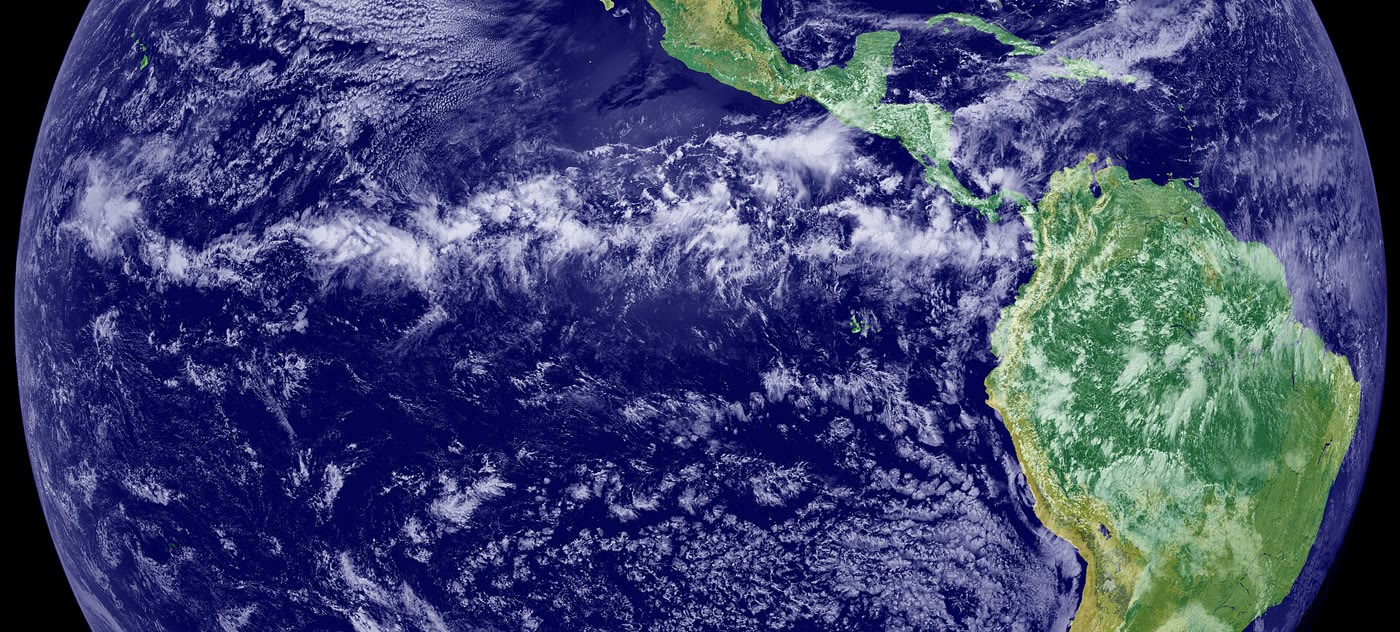
\includegraphics[width=0.8\linewidth]{images/book3/b1-itcz-goes.jpg}

{\small The \omterm{def:b1:atmospheric-circulation:itcz}{intertropical convergence zone} over the eastern Pacific: a line of
bright clouds crossing the ocean north of the equator, with Central and South
America to the right. The image combines cloud data from the GOES-11 geostationary
satellite with colours of the land cover. (NASA Earth Observatory, public domain,
via Wikimedia Commons.)}
\label{fig:b1:atmospheric-circulation:itcz-photo}
\end{omfigure}
% ledger: commons:itcz-goes

Converging air must rise, and rising moist air builds clouds: the ITCZ is the rainiest
belt of the planet, and its position is traced by the \omterm{def:b1:spherical-astronomy:geographic}{latitude} where the zonal-mean
precipitation peaks. The ITCZ follows the Sun, with a delay. In the reanalysis the
peak moves from \ang{12.8} S in February to \ang{10.9} N in September; averaged over
the twelve months it lies at \ang{2.6} N. The zonal mean hides large differences
between \omterm{def:b1:spherical-astronomy:geographic}{longitudes}: over the eastern Pacific in the photograph the band lies north
of the equator, and a zonal mean averages such bands with others that swing farther
with the seasons.
% ledger: data:b3-ncep (computed in figdata/bachelor-1/general_circulation.py)

\begin{omfigure}
\begin{tikzpicture}
\begin{axis}[omrecord, width=0.7\linewidth, height=5.2cm, xmin=0.5, xmax=12.5, ymin=-16, ymax=16,
  xlabel={month}, ylabel={latitude (\unit{\degree})}, xtick={1,...,12},
  xticklabels={J,F,M,A,M,J,J,A,S,O,N,D}, ytick={-15,-10,...,15}]
% figdata/bachelor-1/general_circulation.py; ledger: data:b3-ncep
\addplot[black!40, domain=0.5:12.5] {0};
\addplot[omThm, line width=1.1pt, mark=*, mark size=1.6pt] table[x=month, y=lat] {figdata/out/bachelor-1-general_circulation-itcz.dat};
\end{axis}
\end{tikzpicture}

{\small The \omterm{def:b1:spherical-astronomy:geographic}{latitude} of the zonal-mean precipitation maximum, month by month, between
\ang{20} S and \ang{20} N: the \omterm{def:b1:atmospheric-circulation:itcz}{intertropical convergence zone} migrates north in the
northern summer and south in the southern summer, two or three months behind the
Sun.
NCEP-NCAR Reanalysis~1, means 1991--2020, data provided by the NOAA PSL.}
\label{fig:b1:atmospheric-circulation:itcz}
\end{omfigure}
% ledger: data:b3-ncep

Along the equator itself, where $f = 0$, the air moves straight down the pressure
gradient, and an east--west circulation appears over the Pacific.

\begin{definition}[Walker circulation]\label{def:b1:atmospheric-circulation:walker}
The \emph{Walker circulation}\index{Walker circulation} is the east--west overturning
cell of the atmosphere along the equatorial Pacific: air rises over the warm waters
of the west, around the Maritime Continent, flows east aloft, sinks over the eastern
Pacific and returns westward near the surface with the \omterm{def:b1:atmospheric-circulation:winds}{trade winds}.
\end{definition}
% ledger: climategov:walker

\begin{omfigure}
\begin{tikzpicture}[>={Stealth[length=2mm]}, font=\scriptsize]
  \fill[blue!12] (0,0) rectangle (11,0.45);
  \shade[left color=orange!45, right color=blue!12] (0,0) rectangle (6,0.45);
  \fill[brown!45] (-0.9,0) rectangle (0,0.6);
  \fill[brown!45] (11,0) rectangle (11.9,0.6);
  \node[anchor=north] at (-0.45,-0.05) {Maritime};
  \node[anchor=north] at (-0.45,-0.35) {Continent};
  \node[anchor=north] at (11.45,-0.05) {South};
  \node[anchor=north] at (11.45,-0.35) {America};
  \node[anchor=north] at (5.5,-0.05) {equatorial Pacific Ocean};
  \node at (1.6,0.22) {warm water};
  \foreach \x in {0.6,1.2,1.8} \fill[black!20] (\x,2.6) circle (0.45);
  \foreach \x in {0.9,1.5} \fill[black!25] (\x,3.0) circle (0.4);
  \draw[line width=1.2pt, omThm, ->] (9.5,0.8) -- (2.0,0.8);
  \draw[line width=1.2pt, omThm, ->] (1.2,1.0) -- (1.2,3.0);
  \draw[line width=1.2pt, omThm, ->] (2.0,3.3) -- (9.5,3.3);
  \draw[line width=1.2pt, omThm, ->] (10.3,3.0) -- (10.3,1.0);
  \node[anchor=south] at (5.75,0.85) {trade winds, east to west};
  \node[anchor=south] at (5.75,3.35) {return flow aloft, west to east};
  \node[anchor=west, align=left] at (1.6,1.8) {rising air,\\heavy rain};
  \node[anchor=east, align=right] at (10.0,1.8) {sinking air,\\dry};
\end{tikzpicture}

{\small The \omterm{def:b1:atmospheric-circulation:walker}{Walker circulation} along the equatorial Pacific (schematic; height not
to scale): rising over the warm west, eastward aloft, sinking in the east and back
westward with the \omterm{def:b1:atmospheric-circulation:winds}{trade winds} near the surface.}
\label{fig:b1:atmospheric-circulation:walker}
\end{omfigure}
% ledger: climategov:walker

The \omterm{def:b1:atmospheric-circulation:walker}{Walker circulation} is not steady. When it weakens, the rising motion over the
Maritime Continent weakens and the air there may even sink; when it strengthens,
the rising and the rain over the west increase. These swings, El~Niño and La~Niña,
and the seasonal reversals of the monsoons are the subject of the Year~2 volume.
Over the decades since 1980, the 2021 assessment of the IPCC finds a \emph{very
likely} strengthening of the \omterm{def:b1:atmospheric-circulation:walker}{Walker circulation}, resembling the La~Niña state, and a
westward shift, with \emph{medium confidence} in the size of the changes.
% ledger: climategov:walker, ipcc:hadley-widening

\section{Jet streams}\label{sec:b1:atmospheric-circulation:jets}

\begin{definition}[Jet stream; subtropical and polar-front jets]\label{def:b1:atmospheric-circulation:jet}
A \emph{jet stream}\index{jet stream} is a narrow band of strong wind, normally a
horizontal wind high in the troposphere, whose position changes from day to day. The
\emph{subtropical jet}\index{subtropical jet} blows from the west near the poleward
edge of the \omterm{def:b1:atmospheric-circulation:cells}{Hadley cell}, usually between \ang{20} and \ang{30} of \omterm{def:b1:spherical-astronomy:geographic}{latitude} at heights
of \qtyrange{12}{14}{km}. The \emph{polar-front jet}\index{polar-front jet} blows
from the west above the boundary between polar and subtropical air, between about
\ang{50} and \ang{60}; it is the fast core of the \omterm{def:b1:atmospheric-circulation:winds}{westerlies}, steered by and steering
the depressions and \omterm{def:b1:atmospheric-circulation:cyclone}{anticyclones} of the \omterm{def:b1:spherical-astronomy:geographic}{mid-latitudes}.
\end{definition}
% ledger: nws:jets, noaajs:jet

\omterm{def:b1:atmospheric-circulation:jet}{Jet streams} are typically found around \qty{9}{km}, can reach more than
\qty{440}{km/h}, and are strongest in the winter of each hemisphere, when the contrast
of temperature between the tropics and the pole is largest. The \omterm{def:b1:atmospheric-circulation:jet}{subtropical jet} is
the angular-momentum wind of \cref{prop:b1:atmospheric-circulation:angular-momentum},
tamed by the eddies; it sits at the edge of the \omterm{def:b1:atmospheric-circulation:cells}{Hadley cell}, near \ang{30} in the
winter mean. The \omterm{def:b1:atmospheric-circulation:jet}{polar-front jet} wanders north and south with the passing
depressions, and averaging round the globe smears it out: in the zonal mean of the
northern summer only a weak maximum of \qty{21.6}{m/s} remains near \ang{42.5} N,
and in the southern summer \qty{29.9}{m/s} near \ang{47.5} S. Why the wind increases
with height wherever the temperature falls towards the pole, the thermal wind, is
shown in the Year~3 volume.
% ledger: noaajs:jet, nws:jets, data:b3-ncep-circ (computed in figdata/bachelor-1/general_circulation.py)

\section{Exercises}

\begin{exercise}[$\star$]\label{exo:b1:atmospheric-circulation:1}
Take $\Omega = \qty{7.292e-5}{rad.s^{-1}}$. (a)~Compute the \omterm{def:b1:atmospheric-circulation:coriolis-parameter}{Coriolis parameter} at
\ang{0}, \ang{30}, \ang{45} and \ang{90} N. (b)~Compute the horizontal Coriolis
acceleration of a wind of \qty{10}{m/s} at \ang{45} N and compare it with $g =
\qty{9.81}{m.s^{-2}}$. (c)~In which direction does it point if the wind blows
towards the north?
% ledger: earth:Trot
\end{exercise}

\begin{exercise}[$\star$]\label{exo:b1:atmospheric-circulation:2}
Two isobars \qty{4}{hPa} apart are \qty{400}{km} apart at sea level, where $\rho =
\qty{1.225}{kg.m^{-3}}$. (a)~Compute the acceleration due to the \omterm{def:b1:atmospheric-circulation:pgf}{pressure-gradient
force}. (b)~If nothing else acted, how long would it take to accelerate still air to
\qty{10}{m/s}? (c)~Compare this acceleration with the Coriolis acceleration of a wind
of \qty{10}{m/s} at \ang{45} N, and say what this suggests.
% ledger: ussa76:sea-level, earth:Trot
\end{exercise}

\begin{exercise}[$\star$]\label{exo:b1:atmospheric-circulation:3}
At \ang{40} N, isobars \qty{4}{hPa} apart are \qty{250}{km} apart; take $\rho =
\qty{1.225}{kg.m^{-3}}$. (a)~Compute the \omterm{def:b1:atmospheric-circulation:geostrophic}{geostrophic wind} in \unit{m/s} and in knots
(\qty{1}{kn} = \qty{0.5144}{m/s}). (b)~The low lies to the south. From which
direction does the wind blow? (c)~Describe the wind barb (staff and feathers) a
forecaster would draw.
% ledger: ussa76:sea-level, earth:Trot
\end{exercise}

\begin{exercise}[$\star$]\label{exo:b1:atmospheric-circulation:4}
The reanalysis's annual means give, near the ground, the eastward wind
\qty{-3.5}{m/s} at \ang{15} N, \qty{-4.4}{m/s} at \ang{15} S, \qty{+1.9}{m/s} at
\ang{45} N and \qty{+6.5}{m/s} at \ang{45} S, and the sea-level pressure
\qty{1011.8}{hPa} at \ang{15} N, \qty{1016.8}{hPa} at \ang{30} N and
\qty{1015.8}{hPa} at \ang{45} N. (a)~Name the wind belt at each of the four \omterm{def:b1:spherical-astronomy:geographic}{latitudes}.
(b)~Explain the sign of each wind with the surface branch of a cell. (c)~Where is the
\omterm{def:b1:atmospheric-circulation:cells}{subtropical high} of the Northern Hemisphere according to these pressures?
% ledger: data:b3-ncep-circ
\end{exercise}

\begin{exercise}[$\star\star$]\label{exo:b1:atmospheric-circulation:5}
A pressure gradient of \qty{2}{hPa} per \qty{500}{km}, with $\rho =
\qty{1.225}{kg.m^{-3}}$, is found at \ang{60}, \ang{50}, \ang{30}, \ang{20},
\ang{10} and \ang{5} N. (a)~Compute the \omterm{def:b1:atmospheric-circulation:geostrophic}{geostrophic wind} at each \omterm{def:b1:spherical-astronomy:geographic}{latitude}.
(b)~Real winds of the deep tropics rarely exceed a few metres per second over such
gradients. Explain why the \omterm{def:b1:atmospheric-circulation:geostrophic}{geostrophic balance} fails near the equator, using the
time $1/f$ the Coriolis force needs to turn the wind.
% ledger: ussa76:sea-level, earth:Trot
\end{exercise}

\begin{exercise}[$\star\star$]\label{exo:b1:atmospheric-circulation:6}
(a)~With \cref{prop:b1:atmospheric-circulation:angular-momentum}, compute the wind
of a ring of air that leaves the equator at rest, at \ang{10}, \ang{15}, \ang{20} and
\ang{30}; take $\Omega a_\oplus = \qty{464.6}{m/s}$. (b)~The same for a ring that
starts at rest at \ang{10}, at \ang{15}, \ang{20} and \ang{30}. (c)~The rising branch
of the \omterm{def:b1:atmospheric-circulation:cells}{Hadley cell} is spread over \omterm{def:b1:spherical-astronomy:geographic}{latitudes} rather than placed exactly at the equator.
How does this change the predicted jet?
% ledger: earth:Trot, earth:Rmean
\end{exercise}

\begin{exercise}[$\star\star$]\label{exo:b1:atmospheric-circulation:7}
(a)~A ship in the Northern Hemisphere has the wind from the south-west. Using Buys
Ballot's law, where is the centre of low pressure? (b)~A ship in the Southern
Hemisphere has the wind from the north-west. Where is the low? (c)~Near the ground the
wind crosses the isobars towards low pressure. Does this change your answer to (a)
by turning the direction of the low clockwise or anticlockwise?
% ledger: skybrary:buys-ballot
\end{exercise}

\begin{exercise}[$\star\star$]\label{exo:b1:atmospheric-circulation:8}
(a)~Compute the mass of air between the equator and \ang{30} N and between the
pressure levels \qty{1000}{hPa} and \qty{100}{hPa}, with $a_\oplus = \qty{6371}{km}$
and $g = \qty{9.81}{m.s^{-2}}$. (b)~In the annual mean the reanalysis's northern
\omterm{def:b1:atmospheric-circulation:cells}{Hadley cell} carries \qty{8.7e10}{kg/s}. How long would it take to pass that mass
through the cell once? (c)~Same question with the northern-winter cell,
\qty{21.4e10}{kg/s}.
% ledger: earth:Rmean, data:b3-ncep-circ
\end{exercise}

\begin{exercise}[$\star\star$]\label{exo:b1:atmospheric-circulation:9}
Suppose that under a \omterm{def:b1:atmospheric-circulation:cells}{subtropical high} the air sinks at \qty{1}{cm/s}, and that it is
unsaturated. (a)~How far does it sink in a day? (b)~By how much does it warm in a day,
if nothing else acts, with the \omterm{def:b1:fluid-envelopes-structure:lapse-rate}{dry adiabatic lapse rate} of \qty{9.8}{K/km}? (c)~The
air does not warm by that much day after day. Which process of
\cref{ch:b1:radiation-heat-transport} balances the warming? (d)~Why are many of the
great hot deserts found under these highs?
% ledger: nws:dalr
\end{exercise}

\begin{exercise}[$\star\star\star$]\label{exo:b1:atmospheric-circulation:10}
At \ang{50} N, take $f = \qty{1.117e-4}{s^{-1}}$ and circular isobars of radius
$r = \qty{500}{km}$ (\cref{rem:b1:atmospheric-circulation:gradient}). (a)~Around a
low where the \omterm{def:b1:atmospheric-circulation:geostrophic}{geostrophic wind} would be \qty{15}{m/s}, solve $V^2/r + fV =
f|\vec v_g|$ for the gradient wind $V$. (b)~Around a high, show that $V^2/r - fV + f
|\vec v_g| = 0$ has a solution only if $|\vec v_g| \leq fr/4$, and compute that limit.
(c)~What does (b) imply for the spacing of the isobars near the centre of an
\omterm{def:b1:atmospheric-circulation:cyclone}{anticyclone}, compared with a depression?
\end{exercise}

\begin{exercise}[$\star\star\star$]\label{exo:b1:atmospheric-circulation:11}
(a)~Show that for small $\varphi$ (in radians) the wind of a ring leaving the equator
at rest is $u \approx \Omega a_\oplus\varphi^2$. (b)~Compare the approximation with
the exact formula at \ang{10}, with $\Omega a_\oplus = \qty{464.6}{m/s}$. (c)~The
reanalysis's annual-mean wind at \qty{200}{hPa} peaks at \qty{27.0}{m/s} near
\ang{35} N. At what \omterm{def:b1:spherical-astronomy:geographic}{latitude} would the ring reach this speed? (d)~What does the
answer say about how far the angular-momentum argument can be trusted?
% ledger: earth:Trot, earth:Rmean, data:b3-ncep-circ
\end{exercise}

\begin{exercise}[$\star\star\star$]\label{exo:b1:atmospheric-circulation:12}
The reanalysis's zonal-mean precipitation peaks at the following \omterm{def:b1:spherical-astronomy:geographic}{latitudes}, from
January to December: \ang{-10.5}, \ang{-12.8}, \ang{-5.8}, \ang{-4.6}, \ang{5.5},
\ang{7.3}, \ang{8.6}, \ang{10.4}, \ang{10.9}, \ang{9.1}, \ang{7.4}, \ang{6.2}
(negative: south). (a)~Compute the annual mean and the range. (b)~The subsolar
\omterm{def:b1:spherical-astronomy:geographic}{latitude} is extreme in June and December. By how many months does the ITCZ lag
behind it, and what in the climate system can store heat to cause such a lag?
(c)~Suppose that over one ocean the ITCZ stays north of the equator all year. Explain
how the zonal mean can still cross the equator.
% ledger: data:b3-ncep
\end{exercise}

\section{Problem: Reading a mid-latitude weather map}

\begin{problem}[{Weekend problem --- the wind at a station near \ang{50} N}]
\label{pb:b1:atmospheric-circulation:1}
% values: calc/ch28.py (invented map; jet from data:b3-ncep-circ)
A weather map of the North Atlantic shows, near a station P at \ang{50} N, straight
isobars running west to east, every \qty{4}{hPa}, with the lower pressures to the
north. P lies between the \qty{1004}{hPa} and \qty{1008}{hPa} isobars, which are
\qty{250}{km} apart there; its sea-level pressure is \qty{1006}{hPa} and its air
temperature \qty{10}{\degreeCelsius}. The map is invented, but its numbers are typical.
Use $\Omega = 2\pi/(\qty{23.9345}{h})$, $a_\oplus = \qty{6371}{km}$, $R_d =
\qty{287.05}{J.kg^{-1}.K^{-1}}$ for dry air, \qty{1}{kn} = \qty{0.514444}{m/s}.

\medskip
\noindent\textbf{Part I --- The pressure gradient and the geostrophic wind.}
\begin{enumerate}
  \item Compute the density of the air at P with the ideal-gas law.
  \item Compute the horizontal pressure gradient at P, in \unit{Pa.m^{-1}}.
  \item Compute the acceleration due to the \omterm{def:b1:atmospheric-circulation:pgf}{pressure-gradient force}.
  \item Compute $\Omega$ and the \omterm{def:b1:atmospheric-circulation:coriolis-parameter}{Coriolis parameter} at \ang{50} N.
  \item Compute the \omterm{def:b1:atmospheric-circulation:geostrophic}{geostrophic wind} speed at P.
  \item Express it in knots and in \unit{km/h}.
  \item Show that the time the \omterm{def:b1:atmospheric-circulation:pgf}{pressure-gradient force} alone would need to bring
        still air to the geostrophic speed is $1/f$, and compute it, together with
        the time $2\pi/f$ the Coriolis force takes to turn a wind full circle.
\end{enumerate}

\medskip
\noindent\textbf{Part II --- Direction and hemisphere.}
\begin{enumerate}[resume]
  \item In which direction does the \omterm{def:b1:atmospheric-circulation:pgf}{pressure-gradient force} point at P? In which
        direction does the \omterm{def:b1:atmospheric-circulation:geostrophic}{geostrophic wind} blow, and from which \omterm{def:b1:spherical-astronomy:horizontal}{azimuth} does it
        come?
  \item Check your answer with Buys Ballot's law.
  \item Describe the wind barb drawn at P: the direction of the staff, the number
        of feathers, and the side on which they stand.
  \item Suppose the same isobars, with the low to the north, were found at
        \ang{50} S. From which direction would the wind blow?
  \item With the same density and pressure gradient, compute the \omterm{def:b1:atmospheric-circulation:geostrophic}{geostrophic wind}
        at \ang{30} N and \ang{60} N.
  \item Compute it at \ang{5} N. Is the result believable? Explain.
\end{enumerate}

\medskip
\noindent\textbf{Part III --- The wind at the ground.} An anemometer at P measures a
wind of \qty{9.0}{m/s} crossing the isobars at \ang{25} towards low pressure.
\begin{enumerate}[resume]
  \item Compute the ratio of the observed wind to the \omterm{def:b1:atmospheric-circulation:geostrophic}{geostrophic wind}, and the
        components of the observed wind along and across the isobars.
  \item From which \omterm{def:b1:spherical-astronomy:horizontal}{azimuth} does the observed wind blow?
  \item In the linear-drag model of \cref{prop:b1:atmospheric-circulation:friction},
        what time constant $\tau$ gives the observed angle, and what speed does the
        model then predict? Compare with the observation.
  \item Around a depression of radius \qty{500}{km}, suppose that the air of the
        lowest kilometre flows inwards everywhere with the cross-isobar component
        of question~14 and the density of question~1. Compute the mass of air
        entering the depression per second.
  \item This air must leave through the top of the layer. Compute the mean upward
        velocity there, in \unit{m/s} and in metres per day.
  \item At the \omterm{def:b1:fluid-envelopes-structure:lapse-rate}{dry adiabatic lapse rate} of \qty{9.8}{K/km}, by how much does the
        rising air cool in a day? What weather follows, and what would happen
        under an \omterm{def:b1:atmospheric-circulation:cyclone}{anticyclone} instead?
\end{enumerate}

\medskip
\noindent\textbf{Part IV --- The jet above.} The zonal-mean wind at \qty{200}{hPa} in
the northern winter peaks at \qty{42.3}{m/s} near \ang{30} N (reanalysis means
1991--2020).
\begin{enumerate}[resume]
  \item Compute the eastward speed of the ground at the equator and at \ang{30} N.
  \item A ring of air leaves the equator at rest aloft and keeps its angular
        momentum. Compute its wind at \ang{20} N and \ang{30} N.
  \item Same question at \ang{30} N for a ring that starts at rest at \ang{10} N.
  \item By what factor does the ring of question~21 outrun the observed jet at
        \ang{30} N? Give two reasons why the real jet is slower.
  \item Compute the ratio of the absolute angular momentum per unit mass of the
        observed jet at \ang{30} N to that of air at rest at the equator. What
        fraction has been lost on the way?
  \item What is the \omterm{def:b1:atmospheric-circulation:geostrophic}{geostrophic wind} speed at P, in metres per second, and how does
        the wind measured at the ground compare with it?
\end{enumerate}
\end{problem}
